\section{Input Coordination Protocol} \label{sec:input}

This section introduces the basic workflow of \xxx's \paxos-based input 
coordination protocol in normal case (\S\ref{sec:normal}), describes how it 
handles concurrent connections (\S\ref{sec:concurrent}), presents the leader 
election protocol (\S\ref{sec:election}), and then discusses the reliability 
of our protocol (\S\ref{sec:guarantees}).

\subsection{Normal Case Operations} \label{sec:normal}

\begin{figure}[t]
\centering
\begin{minipage}{.5\textwidth}
\lgrindfile{code/logentry.cpp}
\end{minipage}
\vspace{-.1in}
\caption{{\em \xxx's log entry for each socket call.}} \label{fig:logentry}
\vspace{-.05in}
\end{figure}

\begin{figure}[t]
\centering
\vspace{-0.15in}
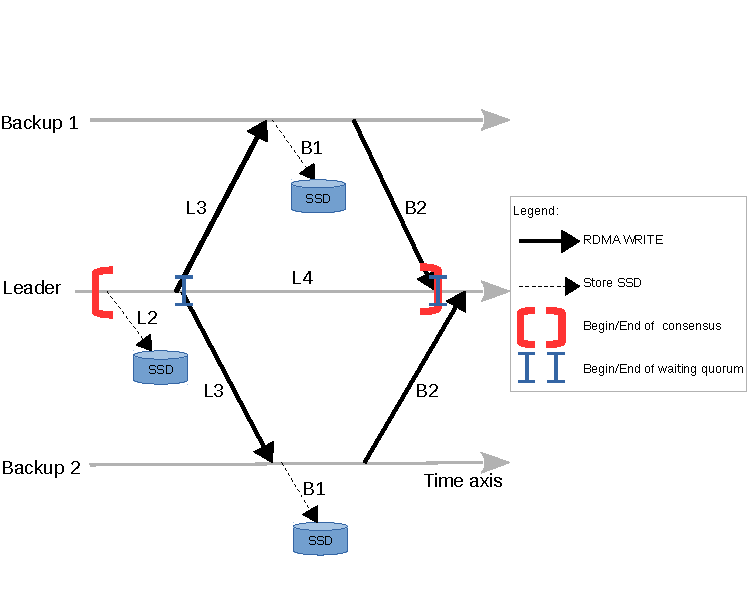
\includegraphics[width=.5\textwidth]{figures/consensus}
\vspace{-.4in}
\caption{{\em \xxx consensus algorithm in normal case.}} \label{fig:consensus}
\vspace{-.05in}
\end{figure}

% \subsubsection{The Basic } \label{sec:primitive}

% Question: What if on a machine, it viewed it as the leader, it executes the 
% actual socket call, and then it invokes the consensus, but then it is no 
% longer the leader any more. How to undo the actual socket calls? Cases:
  %% On accept(). The old leader has already accepted and asks for consensus.
  %% On recv(). The old leader has already received.
  %% On send().
  %% On close().

% First, basic roles. log format details.
\xxx' input coordination protocol contains three roles. The first role is a 
\paxos consensus log (for short, \emph{log}) which resides in each replica and 
contains the same  sequence of socket calls called by a server program. The 
second role is a leader thread which invokes consensus request and writes to its 
local log as well as remote replicas' logs. In \xxx, leader threads are just 
a server program's worker threads that processes client requests. A leader 
replica can have multiple leader threads depending on how many threads  Third, 
a follower thread which (dis)agrees consensus requests on a backup replica.

Figure~\ref{fig:logentry} shows the data structure of a log entry in \xxx's 
consensus log. Most fields are regular as those in a typical \paxos protocol 
except three ones: the \v{ack} array, the client connection ID \v{conn\_vs}, 
and the type ID of a socket call \v{call\_type}. The \v{ack} array is for 
replicas to write back their consensus replies to the leader via a RDMA one-side 
write. The \v{conn\_vs} is for identifying which connection this socket call 
belongs to (see \ref{sec:conclusion}). The \v{call\_type} identifies four types 
of socket calls in \xxx: the \accept type (\eg, \accept), the \recv type 
(\eg, \recv and \myread), the \send type (\eg, \send and \mywrite), and the 
\close type (\eg, \close).

% Second, leader thread behavior on \recv(). Return from orig recv, grab 
% spin % lock and get view stamp, store the log, and post send to all replicas. 
% Non blocking. Wait % for over half agree, and then execute the operation.
A leader thread invokes a consensus request when it calls a socet call with 
the \recv type. A consensus request includes four steps. The first step is 
executing the actual socket call, because \xxx needs to get the actual received 
data bytes and then replicates them in remote replicas' logs.

The second step is local preparation, including assigning a global, 
monotonically increashing viewstamp to locate this entry in the consensus log, 
building a log entry struct for this call, and writing this entry to its local 
SSD.

The third step is sending consensus requests to replicas by using RDMA 
one-sided write to write this struct to remote replicas' logs. Note that these 
RDMA write operations do not need to wait for the struct actually be written to 
remote logs. Instead, \xxx's leader thread just return immediately after 
putting the structs to the RDMA QP (Queue Pair) between a backup replica, 
because \paxos protocol \xxx implements has already considered packet losses 
(\eg, due to remote replica failures).

The fourth step is waiting for replicas' consensus replies. The leader does a
busy loop to check the \v{ack} array until it sees that a majority of replicas, 
including itself, have aggreed on this log entry. In normal case, both the 
third and fourth steps will return immediately because no synchronization 
context switch is involved.

% Post send carry the last committed (consensus reached) operation.

% One key issue, check integrity. Strawmen approach, check viewstamp first.
On a replica side, one tricky issue on replying consensus request is that, 
unlike traditional TCP/UDP messages, RDMA on-sided write operations do not 
guarantee atomicy. For instance, a leader thread can be doing a remote RDMA 
write on the viewstamp \v{vs}, while a follower thread can be reading this 
variable concurrently without knowing when the leader's write can finish, 
causing the replica to read a partial (wrong) value. Thus, in a 
RDMA-accelerated protocol, an extra mechanism is needed to gurantee that a 
leader's write has finished and then replicas can agree or disagree.

\xxx's follower thread tackles this issue by adding a canary value after the 
actual \v{data} array. Leveraging a RDMA feature that its writes are lossless 
in normal case, the follower thread always checks the canary value according to 
\v{data\_size} and then starts the consensus reply decision. This check 
guarantees that a log entry is completely written in a local backup.

To ahchieve small consensus latency, \xxx's follower thread does a busy loop 
on a dedicated CPU core to agree on consensus requests from the leader. Each 
backup only needs one follower thread. This thread always busy reading the 
latest un-agreed log entry in its local log, and it it sees a log entry has 
completely written, it runs three steps. First, it does a regular \paxos view 
ID checking to see whether the leader is up to date, and if so, it stores the 
log entry in its local SSD. Second, it does a RDMA write to send back a Yes/No 
ack to the leader's \v{ack} array element with its own node ID.

Third, the follower thread does a regular \paxos check on \v{last\_committed} 
and executes all socket calls that it has not executed before this viewstamp. 
It ``executes" each log entry by sending the data in each entry to the local 
server program. On replicas, server programs run as is without being 
intercepted. In short, this follower thread runs a high performance loop to 
respond consensus requests and forward data to the local server program. Since 
each backup machine only has one follower thread and nowadays machines often 
have spare cores, we didn't find that the spin loop of this thread brought 
bring negative performance impact in our evaluation.

% Performance: two RDMA writes and two SSD stores. No context switches.
This protocol is highly optimized for minimizing consensus latency in normal 
case. In total, a consensus between the leader and one backup only requires 
two one-sided RDMA write operations (one from the leader to the backup and the 
other from the backup to the leader) and two SSD write operations (each in 
leader and backup). Although each RDMA one-sided operation takes about 3 \us, 
\xxx's protocol just puts the log entry to the RDMA Queue Pair without needing 
to wait until the write succeeds on the remote backup, because the leader will 
have \paxos's consensus reply (the RDMA write from the backup to leader). In 
addition, neither a leader thread or a follower thread does a synchronization 
context switch during this consensus (a synchronization context switch 
typically takes sub milli seconds, pretty slow).

% Question: one key question, can RDMA lose packets in between? I mean, both 
% data_size and canary value are correct, but packets in the middle are lost. 
% This may violate \paxos's non-corrupting packets assumption.

% Third, replica thread behavior on \recv(). Block on latest un agreed log, 
% wait for the % consensus log, check integrity, check view id, and then store to 
% BDB. and % then execute the committed but not executed requests from BDB.

\subsection{Handling Concurrent Connections} \label{sec:concurrent}

Unlike traditional \paxos protocols which mainly handle single-threaded 
programs due to their deterministic state machine assumption, \xxx aims to 
support both single-threaded as well as multithreaded server programs running 
on multi-core machines. Therefore, a strongly consistent mechanism is needed to 
match every concurrent client connection on the leader and to its matching 
connection on replica machines. A naive approach could be matching a leader's 
socket descriptor to the same one on a backup replica, but note that backups' 
servers may return different descriptors because such systems resources could 
be contended by other threads in the server's process and nondeterministic.

Fortunately, \paxos have already made viewstamps of socket calls strongly 
consistent across replicas. For TCP connections, \xxx addes the 
\v{conn\_vs} field, the viewstamp of the the first socket call in each 
connection (aka, \accept) to as the connection ID for socket calls in the 
log. On a local replica, \xxx maintains a hash map between this connection ID 
to the actual local socket descriptor for each connection, then \xxx ensures 
that data bytes are forwarded from a leader's connection to the right matching 
connection on backups. \xxx also intercepts socket calls with the \close type 
to clean up this map. For servers that use UDP to serve requests, \xxx maps the 
viewstamp of a \recvfrom call to the socket descriptor returned from this call, 
and it cleans up the map on a corresponding \sendto call. 

% TBD. Strawmen approach, use fds on leader machines.

%% thread ID mapping is not good too, because accept and recv can be called by 
% different threads in leader side.

% Use viewstamp of the accept() operation, consistent across replicas.


% What does replica thread do. High performance loop on a dedicated core.

\subsection{Leader Election} \label{sec:election}

% % Use one log operation or a few operations to do so. Clean, 
% match the PMS intention. Explain why this design choice is good.

% TBD. Four steps. Four entries?

\subsection{Reliability and Safety} \label{sec:guarantees}

\begin{figure}[t]
\centering
\vspace{-.20in}
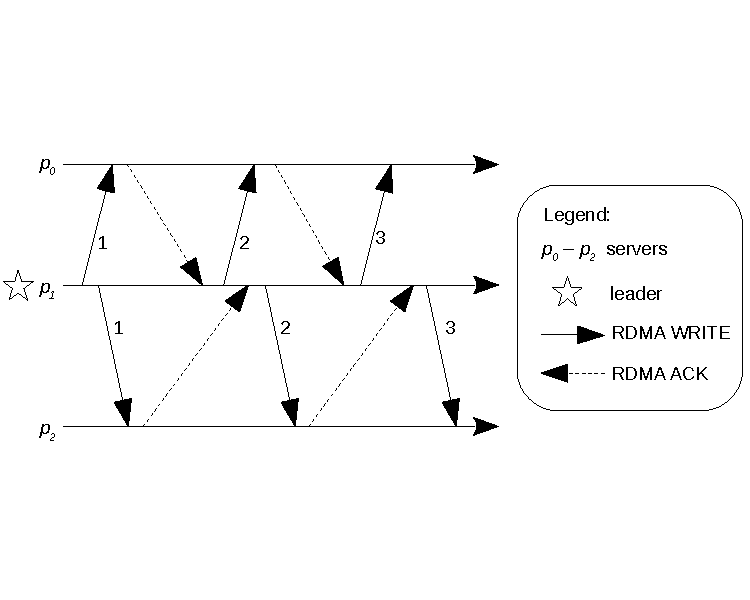
\includegraphics[width=.5\textwidth]{figures/dare}
\vspace{-.20in}
\caption{{\em DARE consensus algorithm in normal case.}} \label{fig:dare}
\vspace{-.05in}
\end{figure}

% Follow PMP, ease to understand, absorbe good exeprience.
To minimize protocol-level software bugs, \xxx's input coordination protocol 
design chooses the same replica behavior as a popular, traditional 
\paxos protocol protocol~\cite{paxos:practical}, although \xxx uses RDMA 
operations to deliver consensus requests and replies and added some extra data 
structure fields. For instance, both \xxx and the 
protocol~\cite{paxos:practical} involve two messages between a leader replica 
and a backup replica in normal case, and they both have the same four steps 
involved by same replica roles on leader election. We made this design choice 
because \paxos is notoriously difficult to understand, test, and verify; 
sticking with a traditional replica behavior helps us incorporate the readily 
mature understanding, engineering experience, and the theoretically verified 
reliability rules~\cite{nsdi07} into our new RDMA-accelerated \paxos protocol.

% Define safety: TBD.
A \paxos protocol must ensure safety: the agreed operation must be an actually 
proposed one; if agreed, all active replicas must consistently enforce this 
operation. Safety is another important sweet spot that \xxx's input 
coordination protocol inherites from traditional \paxos protocol by sticking 
with same replica behavior in traditional ones. As a traditional protocol, 
our input coordination protocol also uses view IDs and viewstamps to enforce a 
consistent, up-to-date leadership across replicas. To address the atomicy issue 
between remote RDMA writes and local memory reads, our protocol addes an 
completion check on log entries (\S\ref{sec:normal}).
% In short, our 
% design choice makes our input coordination protocol enforce the same level of 
% safety as traditional \paxos protocols~\cite{paxos, paxos:simple, 
% paxos:practical}.

% Safety, viewstamp.

% Store to stable storage.

% Any unique changes that prevent us from providing guarantees? The delta 
% changes? Packets. Logs?